\everymath{\displaystyle}
\documentclass{beamer}
% \documentclass[handout]{beamer}

%\usepackage[pdftex]{color,graphicx}
\usepackage{amsmath,amssymb,amsfonts}

\mode<presentation>
{
  % \usetheme{Darmstadt}
  % \usetheme[hideothersubsections]{Hannover}
  % \usetheme[hideothersubsections]{Goettingen}
  \usetheme[hideothersubsections, right]{Berkeley}

  \usecolortheme{seahorse}
  % \usecolortheme{dolphin}
  \usecolortheme{rose}
  % \usecolortheme{orchid}

  \useinnertheme[shadow]{rounded}

  \setbeamercovered{transparent}
  % or whatever (possibly just delete it)
}

\mode<handout>{
  \setbeamercolor{background canvas}{bg=black!5}
  \usepackage{pgfpages}
  \pgfpagesuselayout{4 on 1}[a4paper,border shrink=5mm, landscape]
}

\usepackage[brazilian]{babel}
% or whatever

% \usepackage[latin1]{inputenc}
\usepackage[utf8]{inputenc}
% or whatever

\usepackage{times}
%\usepackage[T1]{fontenc}
% Or whatever. Note that the encoding and the font should match. If T1
% does not look nice, try deleting the line with the fontenc.


\title%[] % (optional, use only with long paper titles)
{Testes não-paramétricos}

\subtitle
{Ou: o que fazer caso seus dados não sejam normais?} % (optional)

\author%[] % (optional, use only with lots of authors)
{Felipe Figueiredo}% \and S.~Another\inst{2}}
% - Use the \inst{?} command only if the authors have different
%   affiliation.

\institute[INTO] % (optional, but mostly needed)
{Instituto Nacional de Traumatologia e Ortopedia
}
  % \inst{1}%
  % Department of Computer Science\\
  % University of Somewhere
  % \and
  % \inst{2}%
  % Department of Theoretical Philosophy\\
  % University of Elsewhere}
% - Use the \inst command only if there are several affiliations.
% - Keep it simple, no one is interested in your street address.

\date%[] % (optional)
{}

% \subject{Talks}
% This is only inserted into the PDF information catalog. Can be left
% out. 



% If you have a file called "university-logo-filename.xxx", where xxx
% is a graphic format that can be processed by latex or pdflatex,
% resp., then you can add a logo as follows:

\pgfdeclareimage[height=1.6cm]{university-logo}{../logo}
\logo{\pgfuseimage{university-logo}}



% Delete this, if you do not want the table of contents to pop up at
% the beginning of each subsection:
\AtBeginSubsection[]
%\AtBeginSection[]
{
  \begin{frame}<beamer>{Sumário}
    \tableofcontents[currentsection,currentsubsection]
  \end{frame}
}


% If you wish to uncover everything in a step-wise fashion, uncomment
% the following command: 

\beamerdefaultoverlayspecification{<+->}


\begin{document}

\begin{frame}
  \titlepage
\end{frame}

\begin{frame}{Sumário}
  \tableofcontents
  % You might wish to add the option [pausesections]
\end{frame}


%% Template
% \section{}

% \subsection{}

% \begin{frame}{}
%   \begin{itemize}
%   \item 
%   \end{itemize}
% \end{frame}

% \begin{frame}
%   \begin{columns}
%     \begin{column}{5cm}
%     \end{column}
%     \begin{column}{5cm}
%     \end{column}
%   \end{columns}
% \end{frame}

% \begin{frame}{}
%   \includegraphics[height=0.4\textheight]{file1}
%   \includegraphics[height=0.4\textheight]{file2}
%   \includegraphics[height=0.4\textheight]{file3}
%   \begin{figure}
%     \caption{}
%   \end{figure}
% \end{frame}

% \begin{frame}{}
%   \begin{definition}
%   \end{definition}
%   \begin{example}
%   \end{example}
%   \begin{block}{Exercício}
%   \end{block}
% \end{frame}

\section{Normalidade}

\subsection{Visualização}

\begin{frame}{Visualização - Histograma}
  \centering
  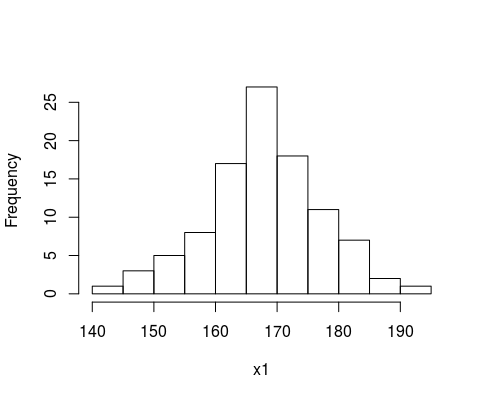
\includegraphics[width=.7\textwidth]{Nao_Param/normal1-h}

  Dados normais
\end{frame}

\begin{frame}{Visualização - Histograma}
  \centering
  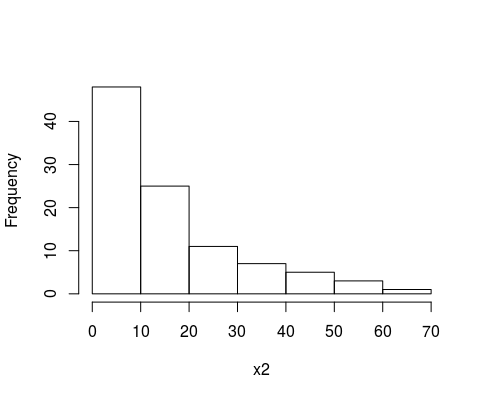
\includegraphics[width=.7\textwidth]{Nao_Param/lognormal1-h}

  Dados não-normais
\end{frame}

\begin{frame}{Visualização - Histograma}
  \centering
  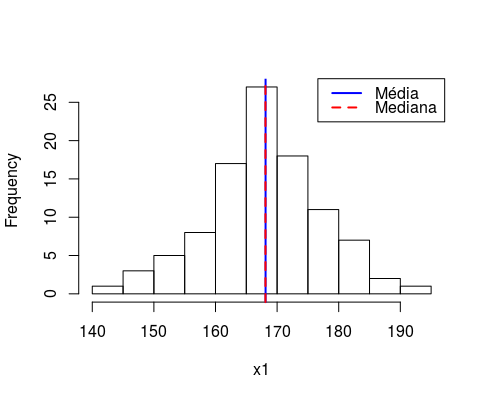
\includegraphics[width=.7\textwidth]{Nao_Param/normal2-h}

  Dados normais
\end{frame}

\begin{frame}{Visualização - Histograma}
  \centering
  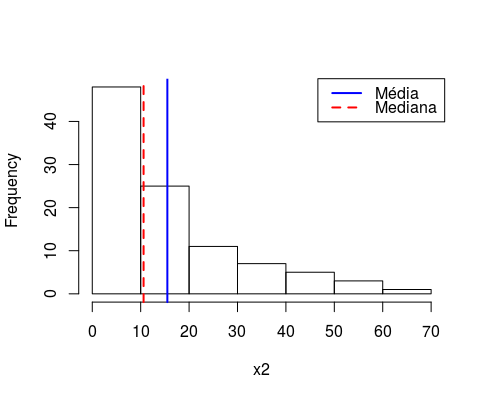
\includegraphics[width=.7\textwidth]{Nao_Param/lognormal2-h}

  Dados não-normais
\end{frame}

\begin{frame}{Visualização - Histograma}
  \centering
  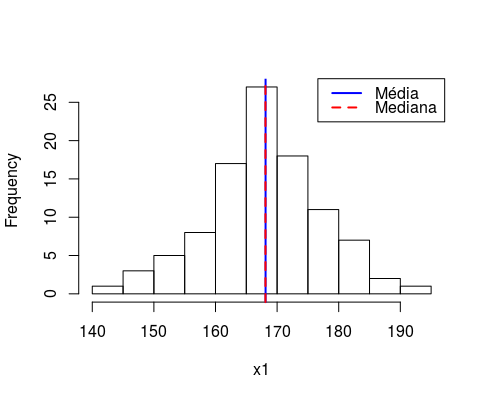
\includegraphics[width=.5\textwidth]{Nao_Param/normal2-h}
  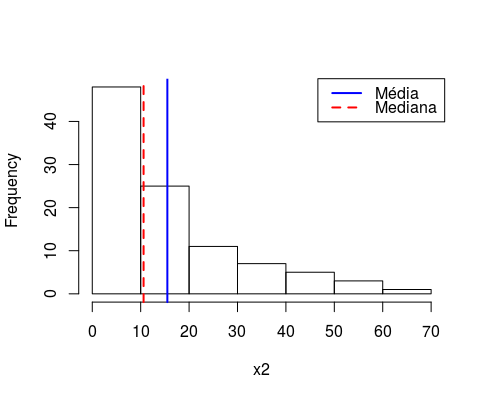
\includegraphics[width=.5\textwidth]{Nao_Param/lognormal2-h}
\end{frame}

\begin{frame}{Visualização - boxplot}
  \centering
  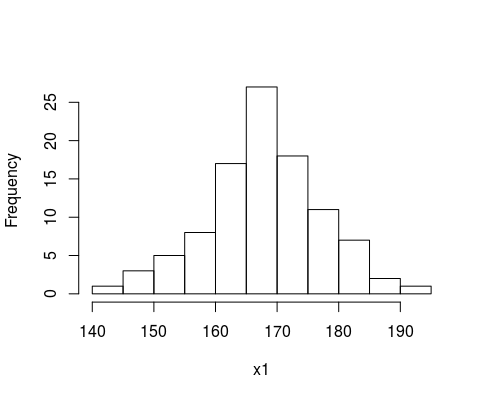
\includegraphics[width=.5\textwidth]{Nao_Param/normal1-h}
  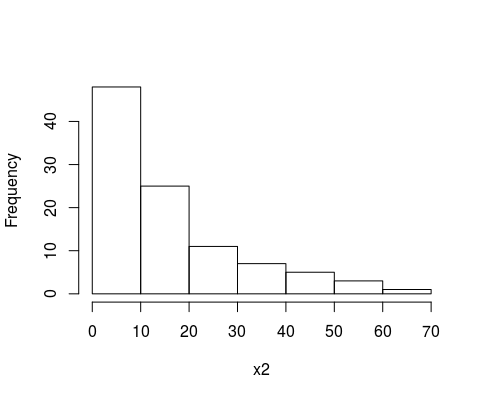
\includegraphics[width=.5\textwidth]{Nao_Param/lognormal1-h}

  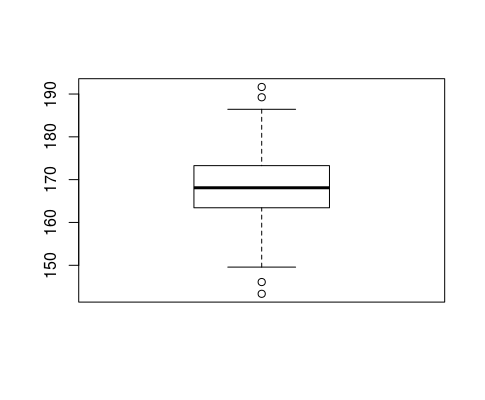
\includegraphics[width=.5\textwidth]{Nao_Param/normal-bp}
  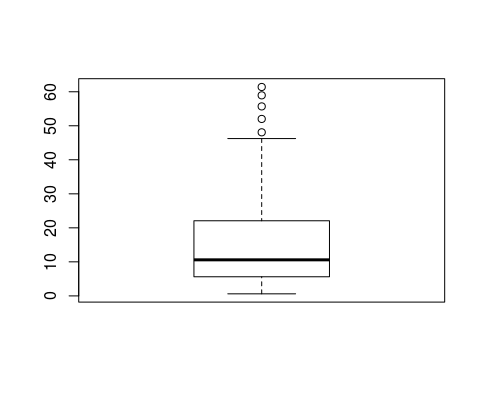
\includegraphics[width=.5\textwidth]{Nao_Param/lognormal-bp}
\end{frame}

\begin{frame}{Visualização - QQ plot}
  \centering
  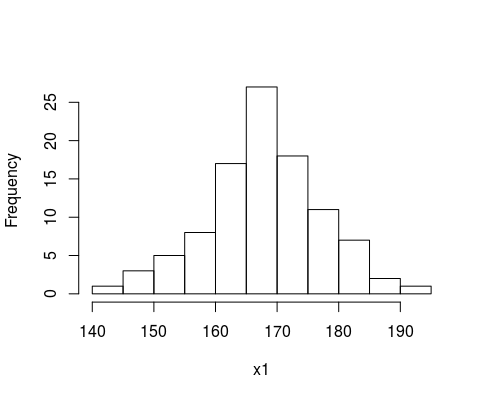
\includegraphics[width=.5\textwidth]{Nao_Param/normal1-h}
  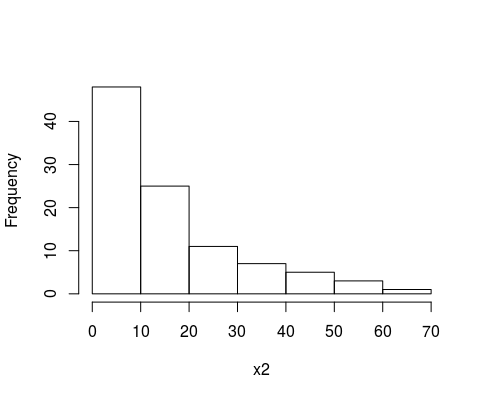
\includegraphics[width=.5\textwidth]{Nao_Param/lognormal1-h}

  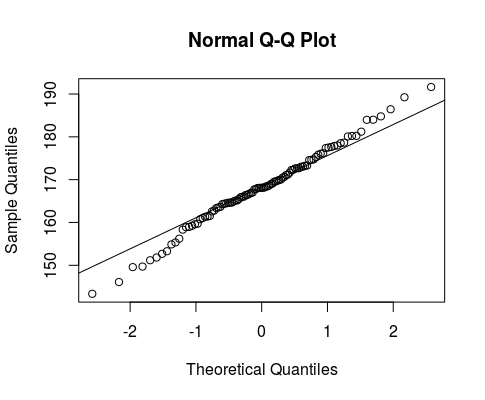
\includegraphics[width=.5\textwidth]{Nao_Param/normal-qq}
  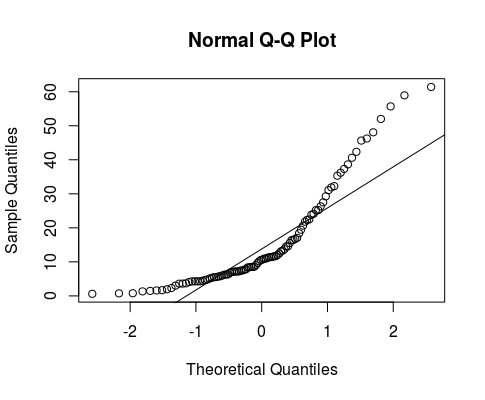
\includegraphics[width=.5\textwidth]{Nao_Param/lognormal-qq}
\end{frame}

\subsection[Normalidade]{Testes contra a normalidade}

\begin{frame}
  \begin{itemize}
  \item Objetivo: é possível \alert{determinar} se uma amostra veio de uma população normalmente distribuída?
  \item Resposta curta: \alert<3->{NÃO}.
  \item<4> Resposta longa: podemos examinar se há evidências para ``aceitar'' esta hipótese\footnote{Lembre que {\bf nunca} aceitamos uma hipótese -- apenas deixamos de rejeitar sua recíproca.}
  \end{itemize}
\end{frame}

\begin{frame}
  \begin{itemize}
  \item Shapiro-Wilk
  \item Anderson-Darling
  \item Kolmongorv-Smirnov
  \end{itemize}
\end{frame}

\section{Testes}

\subsection{Revisão}

\subsection[1 amostra]{Teste para 1 amostra}

\subsection[2 médias]{Testes para 2 amostras}

\begin{frame}{Testes para 2 amostras}
  \begin{block}{Dados normais}
    \begin{itemize}
    \item amostras independentes $\Rightarrow$ t-teste não-pareado
    \item amostras pareadas $\Rightarrow$ t-teste pareado
    \end{itemize}
  \end{block}
  \begin{block}{Dados não-normais}
    \begin{itemize}
    \item amostras independentes $\Rightarrow$ Mann-Whitney \footnote{Também conhecido como Wilcoxon (rank sum test)}
    \item amostras pareadas $\Rightarrow$ Wilcoxon (signed rank test)
    \end{itemize}
  \end{block}
\end{frame}

\begin{frame}{Exemplo}
P: Estas amostras são significativamente diferentes?

  \centering
  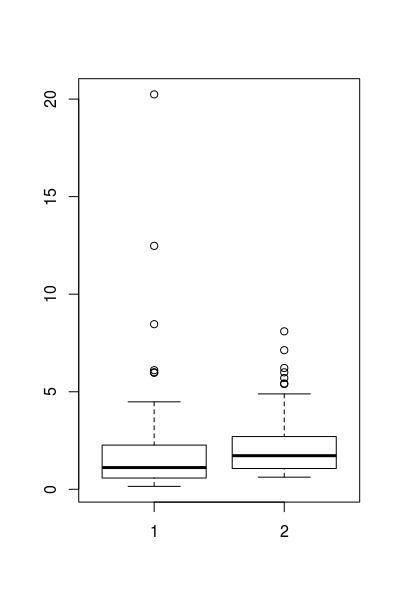
\includegraphics[height=\textheight]{Nao_Param/2samples-bp}
\end{frame}

\begin{frame}{Exemplo}
  \begin{itemize}
  \item Assumindo\footnote{pelo desenho experimental} que elas são independentes, poderíamos fazer um teste t não-pareado.
  \item Resultado: p-valor = \alert{0.259}
  \item Então elas não são diferentes?
  \end{itemize}
\end{frame}

\begin{frame}{Histogramas}
  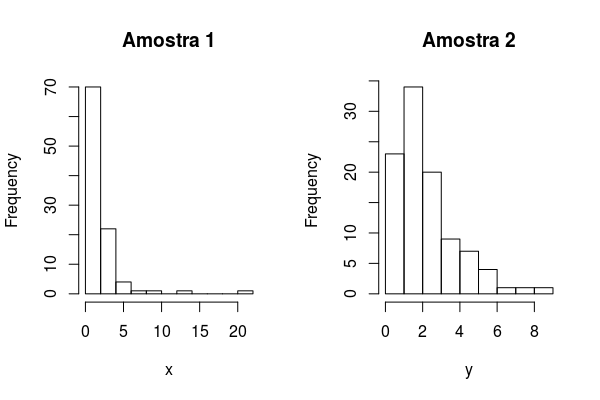
\includegraphics[width=\textwidth]{Nao_Param/2samples-h}

%p-valores Shapiro-Wilk: (x) =  5.515e-16, (y) = 5.274e-09
\end{frame}

\begin{frame}{QQ-plots}
 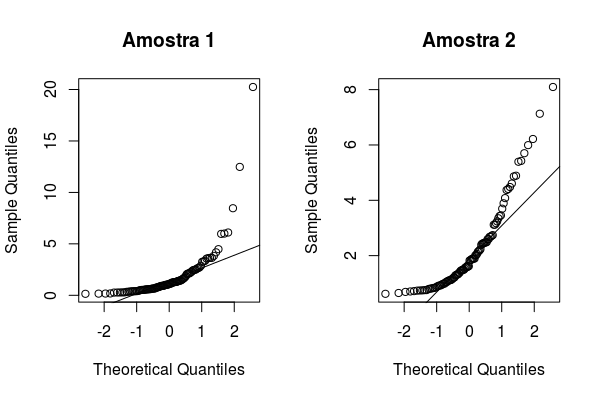
\includegraphics[width=\textwidth]{Nao_Param/2samples-qq}

%p-valores Shapiro-Wilk: (x) =  5.515e-16, (y) = 5.274e-09
\end{frame}

\begin{frame}{Shapiro-Wilk}
  \begin{block}{Teste t}
    p-valor = 0.259 (não são diferentes)
  \end{block}
  \begin{itemize}
  \item<2-> Aplicando o teste de Shapiro-Wilk em x e y
    \begin{itemize}
    \item<2-> x: p-valor = 5.515e-16
    \item<2-> y: p-valor = 5.274e-09
    \end{itemize}
  \item Devemos rejeitar a hipótese de normalidade.
  \item Então o teste t \alert{não é} apropriado!
  \item Substituto: teste de Mann-Whitney
  \end{itemize}
  \begin{block}{Teste de Mann-Whitney}
    p-value = \alert{0.0001346} (são diferentes)
  \end{block}
\end{frame}

\subsection[3+ amostras]{Teste para 3 ou mais amostras}

\subsection[Correlação]{Teste de correlação}

\section{Resumo}

\begin{frame}{Resumo}
  \begin{tabular}{||l||l||}
    \hline
    Paramétrico & Não-paramétrico\\
    \hline
    \hline
    t-teste pareado & Wilcoxon\\
    \hline
    t-teste não-pareado & Mann-Whitney\\
    \hline
    ANOVA 1 fator & Kruskal-Wallis\\
    \hline
    Correlação de Pearson & Correlação de Spearman\\
    \hline
  \end{tabular}

\end{frame}

\end{document}
